\documentclass[a4paper, 11pt]{article}
\usepackage{amsmath}
\usepackage{graphicx}
\usepackage{geometry}
\usepackage{listings}
\geometry{scale=0.8}
\linespread{1.5}
\usepackage{hyperref}
\usepackage{listings}
\usepackage{enumitem}
\setenumerate[1]{itemsep=0pt,partopsep=0pt,parsep=\parskip,topsep=0pt}
\setitemize[1]{itemsep=0pt,partopsep=0pt,parsep=\parskip,topsep=0pt}
\setdescription{itemsep=0pt,partopsep=0pt,parsep=\parskip,topsep=0pt}


\title{	
\normalfont \normalsize
\textsc{School of Computer Science, Sun Yat-sen University} \\ [25pt] %textsc small capital letters
\rule{\textwidth}{0.5pt} \\[0.4cm] % Thin top horizontal rule
\huge  E10 Decision Tree\\ % The assignment title
\rule{\textwidth}{2pt} \\[0.5cm] % Thick bottom horizontal rule
\author{20214810 Suixin Ou}
\date{\normalsize December 14, 2021} 
}

\begin{document}
\maketitle
\tableofcontents
\newpage

\section{Datasets}
\label{sec:datasets}

The UCI dataset (\url{http://archive.ics.uci.edu/ml/index.php}) is the most widely used dataset for machine learning. If you are interested in other datasets in other areas, you can refer to \url{https://www.zhihu.com/question/63383992/answer/222718972}.

Today's experiment is conducted with the \textbf{Adult Data Set} which can be found in \url{http://archive.ics.uci.edu/ml/datasets/Adult}. 
\begin{figure}[ht]
\centering
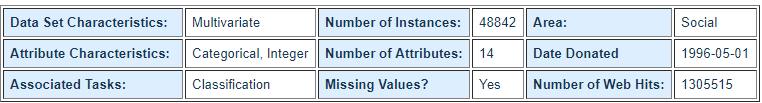
\includegraphics[width=17cm]{dataset.png}
\end{figure}

You can also find 3 related files in the current folder, \texttt{adult.name} is the description of \textbf{Adult Data Set}, \texttt{adult.data} is the training set, and \texttt{adult.test} is the testing set. There are 14 attributes in this dataset:
\begin{lstlisting}{language=Python}
>50K, <=50K.

1. age: continuous.
2. workclass: Private, Self-emp-not-inc, Self-emp-inc, Federal-gov, Local-gov, 
State-gov, Without-pay, Never-worked.
3. fnlwgt: continuous.
4. education: Bachelors, Some-college, 11th, HS-grad, Prof-school, Assoc-acdm, 
Assoc-voc, 9th, 7th-8th, 12th, Masters, 5. 1st-4th, 10th, Doctorate, 5th-6th, 
Preschool.
5. education-num: continuous.
6. marital-status: Married-civ-spouse, Divorced, Never-married, Separated, 
Widowed, Married-spouse-absent, Married-AF-spouse.
7. occupation: Tech-support, Craft-repair, Other-service, Sales, 
Exec-managerial, Prof-specialty, Handlers-cleaners, Machine-op-inspct, 
Adm-clerical,Farming-fishing,Transport-moving,Priv-house-serv,Protective-serv, 
Armed-Forces.
8. relationship: Wife,Own-child,Husband,Not-in-family,Other-relative,Unmarried.
9. race: White, Asian-Pac-Islander, Amer-Indian-Eskimo, Other, Black.
10. sex: Female, Male.
11. capital-gain: continuous.
12. capital-loss: continuous.
13. hours-per-week: continuous.
14. native-country: United-States, Cambodia,England,Puerto-Rico,Canada,Germany, 
Outlying-US(Guam-USVI-etc),India,Japan,Greece, South,China,Cuba,Iran,Honduras, 
Philippines, Italy, Poland, Jamaica, Vietnam, Mexico, Portugal, Ireland, France, 
Dominican-Republic,Laos,Ecuador,Taiwan, Haiti, Columbia,Hungary,Guatemala, 
Nicaragua,Scotland,Thailand,Yugoslavia,El-Salvador, Trinadad&Tobago,Peru,Hong, 
Holand-Netherlands.

\end{lstlisting}
\textbf{Prediction task is to determine whether a person makes over 50K a year.}

\section{Decision Tree}

\subsection{ID3}
ID3 (Iterative Dichotomiser 3) was developed in 1986 by Ross Quinlan. The algorithm creates a multiway tree, finding for each node (i.e. in a greedy manner) the categorical feature that will yield the largest information gain for categorical targets. Trees are grown to their maximum size and then a pruning step is usually applied to improve the ability of the tree to generalise to unseen data.

\textbf{ID3 Algorithm:}
\begin{enumerate}
	\item Begins with the original set $S$ as the root node.
	\item Calculate the entropy of every attribute $a$ of the data set $S$.
	\item Partition the set $S$ into subsets using the attribute for which the resulting entropy after splitting is minimized; or, equivalently, information gain is maximum.
	\item Make a decision tree node containing that attribute.
	\item Recur on subsets using remaining attributes.
\end{enumerate}

\textbf{Recursion on a subset may stop in one of these cases:}
\begin{itemize}
	\item every element in the subset belongs to the same class; in which case the node is turned into a leaf node and labelled with the class of the examples.
	\item there are no more attributes to be selected, but the examples still do not belong to the same class. In this case, the node is made a leaf node and labelled with the most common class of the examples in the subset.
	\item there are no examples in the subset, which happens when no example in the parent set was found to match a specific value of the selected attribute. 
\end{itemize}

\textbf{ID3 shortcomings:}
\begin{itemize}
	\item ID3 does not guarantee an optimal solution. 
	\item ID3 can overfit the training data. 
	\item ID3 is harder to use on continuous data.
\end{itemize}

\textbf{Entropy:}

Entropy $H(S)$ is a measure of the amount of uncertainty in the set $S$.
$$H(S)=\sum_{x\in X}-p(x)\log_2p(x)$$
where
\begin{itemize}
	\item $S$ is the current dataset for which entropy is being calculated
	\item $X$ is the set of classes in $S$
	\item $p(x)$ is the proportion of the number of elements in class $x$ to the number of elements in set $S$.
\end{itemize}

\textbf{Information gain:}

Information gain $IG(A)$ is the measure of the difference in entropy from before to after the set $S$ is split on an attribute $A$. In other words, how much uncertainty in $S$ was reduced after splitting set $S$ on attribute $A$.
$$IG(S,A)=H(S)-\sum_{t\in T}p(t)H(t)=H(S)-H(S\ |\ A)$$
where
\begin{itemize}
	\item $H(S)$ is the entropy of set $S$
	\item T is the subsets created from splitting set $S$ by attribute $A$ such that $S=\cup_{t\in T}t$
	\item $p(t)$ is the proportion of the number of elements in $t$ to the number of elements in set $S$
	\item $H(t)$ is the entropy of subset $t$.
\end{itemize}
\subsection{C4.5 and CART}
C4.5 is the successor to ID3 and removed the restriction that features must be categorical by dynamically defining a discrete attribute (based on numerical variables) that partitions the continuous attribute value into a discrete set of intervals. C4.5 converts the trained trees (i.e. the output of the ID3 algorithm) into sets of if-then rules. These accuracy of each rule is then evaluated to determine the order in which they should be applied. Pruning is done by removing a rule’s precondition if the accuracy of the rule improves without it.

C5.0 is Quinlan’s latest version release under a proprietary license. It uses less memory and builds smaller rulesets than C4.5 while being more accurate.

CART (Classification and Regression Trees) is very similar to C4.5, but it differs in that it supports numerical target variables (regression) and does not compute rule sets. CART constructs binary trees using the feature and threshold that yield the largest information gain at each node.


\section{Tasks}
\begin{itemize}
\item Given the training dataset \texttt{adult.data} and the testing dataset \texttt{adult.test}, please accomplish the prediction task to determine whether a person makes over 50K a year in \texttt{adult.test} by using ID3 (or C4.5, CART) algorithm (C++ or Python), and compute the accuracy. 
\begin{enumerate}
\item You can process the continuous data with \textbf{bi-partition} method.
\item You can use prepruning or postpruning to avoid the overfitting problem.
\item You can assign probability weights to solve the missing attributes (data) problem.
\end{enumerate}

\item Please finish the experimental report named \texttt{E10\_YourNumber.pdf}, and send it to \texttt{ai\_2021@foxmail.com}
\end{itemize}

\section{Codes and Results}


%\clearpage
%\bibliography{E:/Papers/LiuLab}
%\bibliographystyle{apalike}
\end{document} 
%%% Local Variables:
%%% mode: latex
%%% TeX-master: t
%%% End:
